\documentclass{article}[12pt]
%\usepackage{fullpage}
%\usepackage{fullpage}
\usepackage{amsmath}
\usepackage{latexsym}
\usepackage{amssymb,amsfonts}
\usepackage{graphicx}
\usepackage{graphics}
\usepackage[margin=.75in]{geometry}

\graphicspath{ {../../images/} }

\begin{document}
\newcommand{\activityname}{
  Know When to Fold 'Em
}
\newcommand{\subtitle}{
  Ge-Origam-itry
}
\phantom{.}\hspace{-.5in}\begin{tabular}{lr}
 \begin{tabular}{l}
    
\includegraphics[width=2in]{AUExploreLogo.pdf}
 \end{tabular}
 & \hspace{.5in}
 \begin{tabular}{r}
    {\Huge \activityname}
 \end{tabular}
\end{tabular}
\thispagestyle{empty}

\noindent\hrulefill
\phantom{.}\vspace{.15in}

Working with other students from your school and an AU Explore volunteer, you'll be creating \textbf{Sonobe Units} which can be combined to create complex three-dimensional geometrical solids called \textbf{polyhedra}.

\begin{figure}[h]
\begin{center}
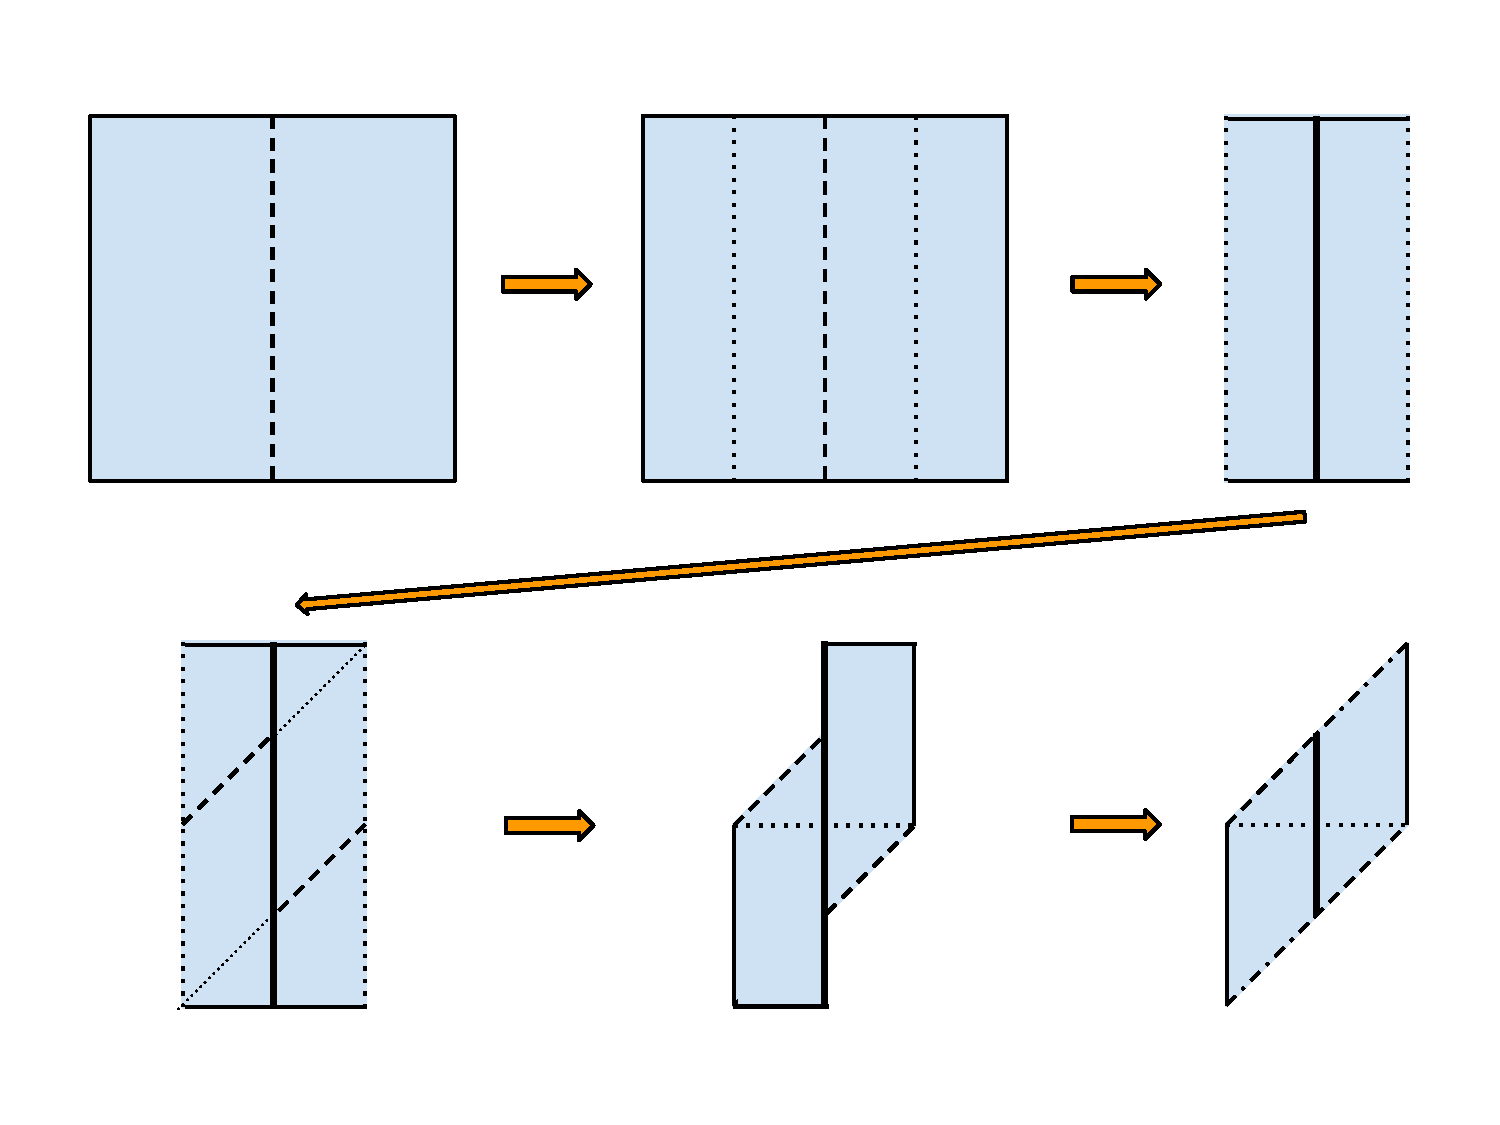
\includegraphics[width=4.4in]{SonobeUnit.pdf}
\end{center}
\end{figure}

While you will use these units today to create simple \textbf{convex} cubes, Sonobe Units are very versitile and can be used to create \textbf{nonconvex} polyhedra as well:

\begin{figure}[h]
\begin{center}
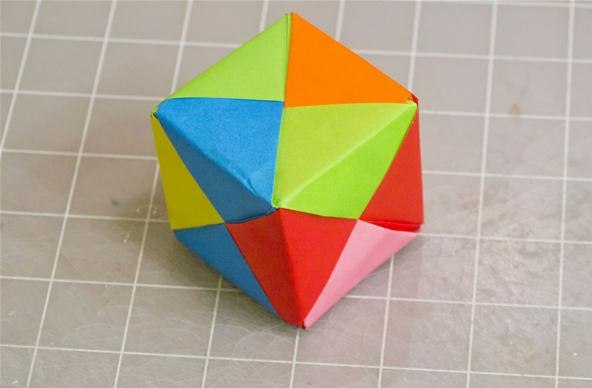
\includegraphics[height=2in]{CubeSonobe.jpg}\hspace{0.3in}
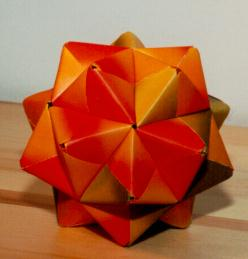
\includegraphics[height=2in]{NonconvexSonobe.jpg}
\end{center}
\end{figure}


\end{document}
